\documentclass{beamer}
\usetheme[numbering=progressbar]{focus}
\usepackage{tikz}
\usetikzlibrary{positioning}
\usetikzlibrary{shapes,arrows}
\usepackage{transparent}
\usepackage{fancyvrb}
\usepackage{listings}
\definecolor{main}{RGB}{47, 161, 219}
%\definecolor{textcolor}{RGB}{128, 128, 128}
\definecolor{background}{RGB}{240, 247, 255}
\definecolor{textcolor}{RGB}{85, 87, 83}
\title{Snake Oil Crypto:}
\subtitle{How I stopped to worry and started to love crypto}
\author{Jean-Louis Huynen}
\titlegraphic{
\includegraphics[scale=0.20]{../../logos/d4-logo.pdf}}
\institute{Team CIRCL \\ \url{https://www.d4-project.org/}}
\date{2019/11/27}

\begin{document}
    \begin{frame}
        \maketitle
    \end{frame}

\begin{frame}
        \frametitle{Outline}

        \begin{itemize}
          \item Cryptography 101,
          \item Cryptography and Network captures,
          \item D4 passiveSSL Collection,
          \item Leveraging OpenPGP metedata,
          \item Checking for weak crypto.
        \end{itemize}

\end{frame}

\begin{frame}
  \begin{center}
    {\bf Cryptography 101}
  \end{center}
\end{frame}


\begin{frame}
  \frametitle{Cryptography Concepts}
        \begin{itemize}
          \item {\bf Plaintext} P: Text in clear,
          \item {\bf Encryption} E: Process of disguising the plaintext to hide its content,
          \item {\bf Ciphertext} C: Result of the Encryption process,
          \item {\bf Decryption} D: Process of reverting encryption, transforming C
            into P,
          \item {\bf Encryption Key} EK: Key to encrypt P into C,
          \item {\bf Decryption Key} DK: Key to decrypt C into P,
          \item {\bf Cryptanalysis}: Analysis of C to recover P without knowing K.
        \end{itemize}

\end{frame}

\begin{frame}
        \frametitle{Cryptography Services}

        \begin{itemize}
          \item {\bf Confidentiality }: Ensure the secrecy of the message except for
            the {\bf intended } recipient,
          \item {\bf Authentication }: Proving a party's identity,
          \item {\bf Integrity }: Verifying that data transmitted were not altered in
            the process,
          \item {\bf Non-repudiation }: Proving that the sender sent a given message.
        \end{itemize}

\end{frame}

\begin{frame}
        \frametitle{Type of Encryption Applications}

        \begin{itemize}
          \item {\bf In-transit encryption}: protects data while it is
            transfered from one machine to another,
          \item {\bf At-rest encryption}: protects data stored on one machine.
        \end{itemize}

\end{frame}

\begin{frame}
        \frametitle{Attack Models}

        \begin{itemize}
          \item
        \end{itemize}

\end{frame}

\begin{frame}
        \frametitle{Kerckhoffs's Principle}

        \begin{itemize}
          \item
        \end{itemize}

\end{frame}




\begin{frame}
        \frametitle{Security Notions}

        \begin{itemize}
          \item
        \end{itemize}

\end{frame}

\begin{frame}
        \frametitle{}

        \begin{itemize}
          \item
        \end{itemize}

\end{frame}


\begin{frame}
  \begin{center}
    {\bf Cryptography and Network captures}
  \end{center}
\end{frame}

\begin{frame}
  \begin{center}
    {\bf D4 passiveSSL Collection}
  \end{center}
\end{frame}

\begin{frame}
  \begin{center}
    {\bf Leveraging OpenPGP metedata}
  \end{center}
\end{frame}

\begin{frame}
  \begin{center}
    {\bf Checking for weak crypto}
  \end{center}
\end{frame}

\begin{frame}
  \frametitle{Snake Oil Crypto\footnote{\url{https://github.com/d4-project/snake-oil-crypto}} - Problem Statement}
  IoT devices {\bf are often the weakest devices} on a network:
        \begin{itemize}
        \item Usually the result of cheap engineering,
        \item sloppy patching cycles,
        \item sometimes forgotten--not monitored,
        \item few hardening features enabled.
        \end{itemize}

        \vspace{10 mm} 

{\bf We feel a bit safer when they use TLS, but should we?}

\end{frame}

\begin{frame}
  \frametitle{Snake Oil Crypto - TLS Fingerprinting}
        {\bf Keep} a log of links between:
        \begin{itemize}
          \item x509 certificates,
          \item ports,
          \item IP address,
          \item client (ja3),
          \item server (ja3s),
        \end{itemize}
        \begin{displayquote}
        ``JA3 is a method for creating SSL/TLS client fingerprints that should be easy to produce on any platform and can be easily shared for threat intelligence.''\footnote{https://github.com/salesforce/ja3}
        \end{displayquote}

         {\bf Pivot} on additional data points during Incident Response 
\end{frame}

\begin{frame}
   \frametitle{Snake Oil Crypto -  Objectives}
   {\bf Collect} and {\bf store} x509 certificates and TLS sessions:
        \begin{itemize}
        \item Public keys type and size,
        \item moduli and public exponents,
        \item curves parameters.
        \end{itemize}
        {\bf Detect} anti patterns in crypto:
        \begin{itemize}
          \item Moduli that share one prime factor,
          \item Moduli that share both prime factors, or private exponents,
          \item Small factors,
          \item Nonces reuse / common preffix or suffix, etc. 
        \end{itemize}
        \vspace{5 mm}
        {\bf Focus on low hanging fruits that appeal to attackers}
\end{frame}


\begin{frame}[fragile]
   \frametitle{Snake Oil Crypto - RSA on IoT }
   Researchers have shown that several devices generated their keypairs
   at boot time without enough entropy\footnote{Bernstein, Heninger, and Lange: \url{http://facthacks.cr.yp.to/}}:
   
\begin{lstlisting}[frame=single, language=python]
prng.seed(seed)
p = prng.generate_random_prime()
// prng.add_entropy()
q = prng.generate_random_prime()
n = p*q
\end{lstlisting}

Given n=pq and n' = pq' it is trivial to recover the shared p by computing their
{\bf Greatest Common Divisor (GCD)}, and therefore {\bf both private keys}\footnote{\url{http://www.loyalty.org/~schoen/rsa/}}.

\end{frame}

\begin{frame}
   \frametitle{Snake Oil Crypto - GCD}
   In Snake-Oil-Crypto we compute GCD\footnote{using Bernstein's Batch GCD algorithm} between:
   
   \begin{itemize}
     \item between certificates having the same issuer,
     \item between certificates having the same subject,
     \item on keys collected from various sources (PassiveSSL, Certificate Transparency,
       shodan, censys, etc.),
   \end{itemize}

\vspace{10 mm}
  {\bf ``Check all the keys that we know of for vendor X''}

\end{frame}

\begin{frame}
   \frametitle{Snake Oil Crypto - MISP feed}
\begin{figure}
\centering
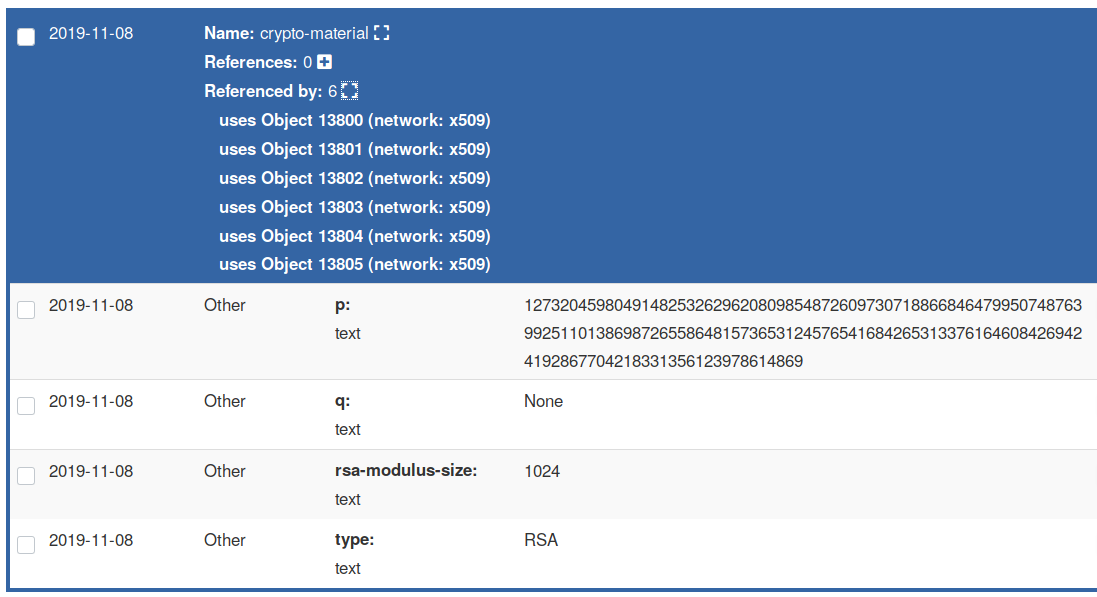
\includegraphics[width=\textwidth]{misp.png}
\end{figure}

\end{frame}

\begin{frame}
   \frametitle{Snake Oil Crypto - MISP feed}
   The MISP feed:
   \begin{itemize}
     \item {\bf Allows} for checking automatic checking by an IDS on hashed values,
     \item {\bf contains} thousands on broken keys from a dozen of vendors,
     \item {\bf will be accessible upon request (info@circl.lu).}
   \end{itemize}

   In the future:
    \begin{itemize}
     \item {\bf Automatic} the vendor checks by performing TF-IDF on x509's subjects, 
     \item {\bf automatic} vendors notification.
     \end{itemize}

\end{frame}


\begin{frame}
  \frametitle{First release}
  \begin{itemize}
  \item[\checkmark] sensor-d4-tls-fingerprinting
    \footnote{\url{github.com/D4-project/sensor-d4-tls-fingerprinting}}:
    {\bf Extracts} and {\bf fingerprints} certificates, and {\bf computes} TLSH fuzzy hash.
  \item[\checkmark] analyzer-d4-passivessl
    \footnote{\url{github.com/D4-project/analyzer-d4-passivessl}}:
    {\bf Stores} Certificates / PK details in a PostgreSQL DB.
  \item snake-oil-crypto 
    \footnote{\url{github.com/D4-project/snake-oil-crypto}}:
    {\bf Performs} crypto checks, push results in MISP for notification
  \item lookup-d4-passivessl
    \footnote{\url{github.com/D4-project/lookup-d4-passivessl}}:
    {\bf Exposes} the DB through a public REST API.
  \end{itemize}
\end{frame}



\begin{frame}
\frametitle{Get in touch if you want to join/support the project, host a passive ssl sensor or contribute}
\begin{itemize}
\item Collaboration can include research partnership, sharing of collected streams or improving the software.
\item Contact: info@circl.lu
\item \url{https://github.com/D4-Project} -  \url{https://twitter.com/d4_project}
\end{itemize}
\end{frame}

\nocite{*} 
\begin{frame}[allowframebreaks]
        \frametitle{References}
        \bibliographystyle{amsalpha}
        \bibliography{../references.bib}
\end{frame}

\end{document}
